\documentclass{article}\usepackage[]{graphicx}\usepackage[]{color}
%% maxwidth is the original width if it is less than linewidth
%% otherwise use linewidth (to make sure the graphics do not exceed the margin)
\makeatletter
\def\maxwidth{ %
  \ifdim\Gin@nat@width>\linewidth
    \linewidth
  \else
    \Gin@nat@width
  \fi
}
\makeatother

\definecolor{fgcolor}{rgb}{0.345, 0.345, 0.345}
\newcommand{\hlnum}[1]{\textcolor[rgb]{0.686,0.059,0.569}{#1}}%
\newcommand{\hlstr}[1]{\textcolor[rgb]{0.192,0.494,0.8}{#1}}%
\newcommand{\hlcom}[1]{\textcolor[rgb]{0.678,0.584,0.686}{\textit{#1}}}%
\newcommand{\hlopt}[1]{\textcolor[rgb]{0,0,0}{#1}}%
\newcommand{\hlstd}[1]{\textcolor[rgb]{0.345,0.345,0.345}{#1}}%
\newcommand{\hlkwa}[1]{\textcolor[rgb]{0.161,0.373,0.58}{\textbf{#1}}}%
\newcommand{\hlkwb}[1]{\textcolor[rgb]{0.69,0.353,0.396}{#1}}%
\newcommand{\hlkwc}[1]{\textcolor[rgb]{0.333,0.667,0.333}{#1}}%
\newcommand{\hlkwd}[1]{\textcolor[rgb]{0.737,0.353,0.396}{\textbf{#1}}}%

\usepackage{framed}
\makeatletter
\newenvironment{kframe}{%
 \def\at@end@of@kframe{}%
 \ifinner\ifhmode%
  \def\at@end@of@kframe{\end{minipage}}%
  \begin{minipage}{\columnwidth}%
 \fi\fi%
 \def\FrameCommand##1{\hskip\@totalleftmargin \hskip-\fboxsep
 \colorbox{shadecolor}{##1}\hskip-\fboxsep
     % There is no \\@totalrightmargin, so:
     \hskip-\linewidth \hskip-\@totalleftmargin \hskip\columnwidth}%
 \MakeFramed {\advance\hsize-\width
   \@totalleftmargin\z@ \linewidth\hsize
   \@setminipage}}%
 {\par\unskip\endMakeFramed%
 \at@end@of@kframe}
\makeatother

\definecolor{shadecolor}{rgb}{.97, .97, .97}
\definecolor{messagecolor}{rgb}{0, 0, 0}
\definecolor{warningcolor}{rgb}{1, 0, 1}
\definecolor{errorcolor}{rgb}{1, 0, 0}
\newenvironment{knitrout}{}{} % an empty environment to be redefined in TeX

\usepackage{alltt}
\IfFileExists{upquote.sty}{\usepackage{upquote}}{}
\begin{document}
\title{Lab 1 - Redwood Data\\
Stat 215A, Fall 2015}
\author{Kuan-Cheng Lai\\25932011}

\maketitle

\section{Introduction}
The redwood dataset was collected by 4 different sensors which are installed in a mote. They deployed those motes around the tree and try to capture the microclimate surrounding the tree over time. Even though the data they collected have a bunch of miss values and unreasonable data, this dataset still contain a lot of informative data point to explore.
\section{The Data}
\subsection{Data Collection}
The data was collected by a set of nodes installed around the 70-meter tall redwood. Each node has 4 sensors which are for temperature, humidity, incident and reflected photosynthetically active solar radiation. They collected data for every 5 minutes for 44 days.\\
\\
Those nodes are actually deployed under certain strategy. They started the deployment 15m from the group with roughly a 2-meter spacing between each node. They also put most of the nodes on the west side of the tree to provide buffer against the environmental effects. Lastly, those nodes are placed 0.1-1.0m from the truch in order to clearly get the microclimate trend that affects the tree. \\

The data was returned by two ways. One way is that the network of sensors tracked each sensor's reading and returned it, while the other is that the data was returned by a local logger which stored the data in a 512KB disk installed on the mote. By doing so, we can make sure one way can compensate for the other way if having some data transmission issues. 

\subsection{Data Cleaning}
First, I checked the whole readings and found out that there were 12532 missing readings which meant that those readings cannot bring us any information we want to measure. Hence, I delted all of them for my first step. Second, as the paper mentioned, when node's voltage fell out of the range of 2.4-3, it started to generate some unreasonable readings. Hence, I ploted the scatter plot with temperature over voltage lower than 2.4 or higher than 3 which are presented respectively by figure 1 and figure 2.
\begin{knitrout}
\definecolor{shadecolor}{rgb}{0.969, 0.969, 0.969}\color{fgcolor}\begin{figure}[h!]

{\centering 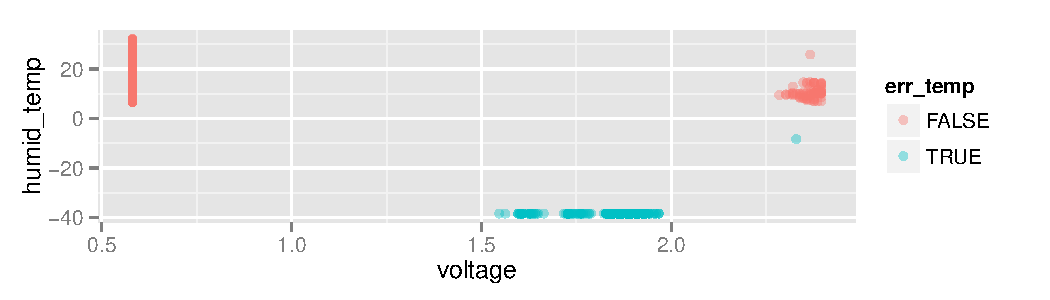
\includegraphics[width=\maxwidth]{figure/addfigure1-1} 

}

\caption[Scatter plot of temperature over voltage lower than 2]{Scatter plot of temperature over voltage lower than 2.4}\label{fig:addfigure1}
\end{figure}


\end{knitrout}
\begin{knitrout}
\definecolor{shadecolor}{rgb}{0.969, 0.969, 0.969}\color{fgcolor}\begin{figure}[h!]

{\centering 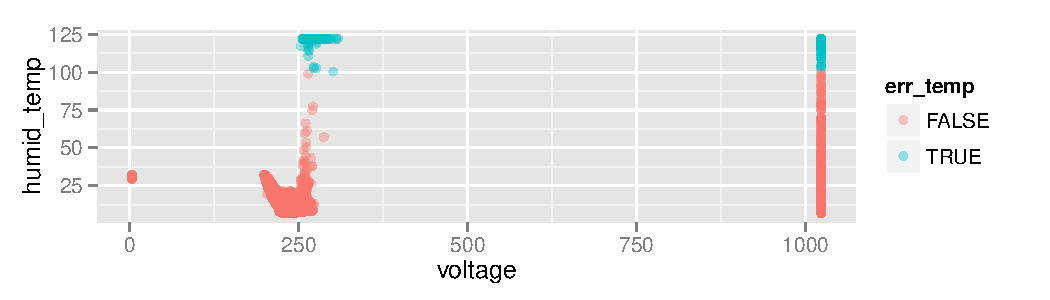
\includegraphics[width=\maxwidth]{figure/addfigure2-1} 

}

\caption[Scatter plot of temperature over voltage larger than 3]{Scatter plot of temperature over voltage larger than 3}\label{fig:addfigure2}
\end{figure}


\end{knitrout}
We can clearly found from this two figures that some erroneous readings like temperature larger than 100C were generated once the voltage fell out of maximum and minimum range. Therefore, I think those data generated under this situation are dubious to use them to analyze. So I delted them at second step. After deleting those data, we can find figure 3 below that all the data of temperature were in the normal range. We also can see most of the variables fell within normal range after the deletion.
\begin{knitrout}
\definecolor{shadecolor}{rgb}{0.969, 0.969, 0.969}\color{fgcolor}\begin{figure}[h!]

{\centering \includegraphics[width=\maxwidth]{figure/addfigure3-1} 

}

\caption[Scatter plot of temperature over voltage]{Scatter plot of temperature over voltage}\label{fig:addfigure3}
\end{figure}

\begin{kframe}\begin{verbatim}
##                      result_time         epoch           nodeid      
##  2004-11-10 14:25:00       :263425   Min.   :    2   Min.   :  2.00  
##  2004-05-07 18:24:58.666424:     0   1st Qu.: 1162   1st Qu.: 46.00  
##  2004-05-07 18:24:58.805974:     0   Median : 2421   Median : 80.00  
##  2004-05-07 18:24:59.075427:     0   Mean   : 3344   Mean   : 87.79  
##  2004-05-07 18:24:59.355354:     0   3rd Qu.: 5274   3rd Qu.:119.00  
##  2004-05-07 18:24:59.675467:     0   Max.   :12635   Max.   :200.00  
##  (Other)                   :     0                                   
##      parent         voltage          depth           humidity     
##  Min.   :    0   Min.   :2.405   Min.   :  1.00   Min.   : 16.27  
##  1st Qu.:   44   1st Qu.:2.651   1st Qu.:  2.00   1st Qu.: 40.33  
##  Median :  118   Median :2.712   Median :  3.00   Median : 61.73  
##  Mean   : 2449   Mean   :2.722   Mean   : 40.38   Mean   : 61.68  
##  3rd Qu.:  140   3rd Qu.:2.788   3rd Qu.: 20.00   3rd Qu.: 80.25  
##  Max.   :65535   Max.   :3.000   Max.   :255.00   Max.   :104.41  
##                                                                   
##    humid_temp       humid_adj         hamatop          hamabot      
##  Min.   : 6.582   Min.   : 16.23   Min.   :     0   Min.   :   0.0  
##  1st Qu.:10.914   1st Qu.: 39.82   1st Qu.:     0   1st Qu.:   0.0  
##  Median :14.736   Median : 60.13   Median :     0   Median :   0.0  
##  Mean   :15.140   Mean   : 59.79   Mean   : 11074   Mean   : 267.4  
##  3rd Qu.:18.822   3rd Qu.: 77.28   3rd Qu.:  6886   3rd Qu.:   0.0  
##  Max.   :32.581   Max.   :100.22   Max.   :180255   Max.   :9142.9  
## 
\end{verbatim}
\end{kframe}
\end{knitrout}
Lastly, we can find that there were a lot of duplicates nodeid with corresponding epoch. Most of these duplicates reading could be slightly different and actuallty I think we have no jugements on which one to use. Therefore, I took average of those duplicates as my last step.

\begin{knitrout}
\definecolor{shadecolor}{rgb}{0.969, 0.969, 0.969}\color{fgcolor}\begin{kframe}
\begin{verbatim}
## Source: local data frame [2 x 2]
## 
##   n  total
## 1 1 246937
## 2 2   8244
\end{verbatim}
\end{kframe}
\end{knitrout}
\subsection{Data Exploration}
First, I explored the range of each variables using kernel density instead of histogram used on the paper. Since I learned that the shape of histogram could change once we use different set of bins, I think kernel estimation could better capture the pattern of the trend. In figure 4 and 5, we found that temperature and relative humidity all showed tri models, we guessed it probabaly has something
related to each other. We assume that lower temperature can cause higher relative humidity
if the moisture stays the same which can be supported by figure 8 below. We can see that clearly temperature and humidity have a negative relationship.

\begin{knitrout}
\definecolor{shadecolor}{rgb}{0.969, 0.969, 0.969}\color{fgcolor}\begin{figure}[h!]

{\centering 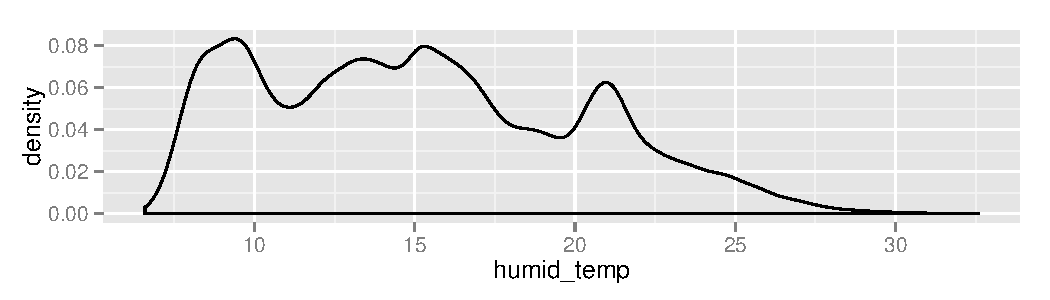
\includegraphics[width=\maxwidth]{figure/addfigure4-1} 

}

\caption[Density plot of temperature]{Density plot of temperature}\label{fig:addfigure4}
\end{figure}


\end{knitrout}

\begin{knitrout}
\definecolor{shadecolor}{rgb}{0.969, 0.969, 0.969}\color{fgcolor}\begin{figure}[h!]

{\centering 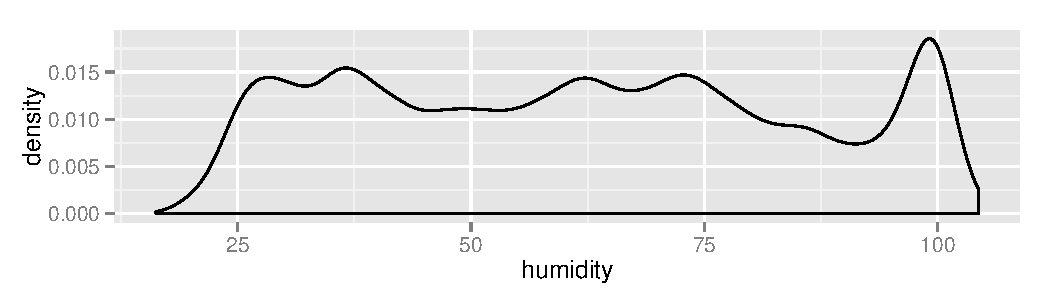
\includegraphics[width=\maxwidth]{figure/addfigure5-1} 

}

\caption[Density plot of humidity]{Density plot of humidity}\label{fig:addfigure5}
\end{figure}


\end{knitrout}

\begin{knitrout}
\definecolor{shadecolor}{rgb}{0.969, 0.969, 0.969}\color{fgcolor}\begin{figure}[h!]

{\centering 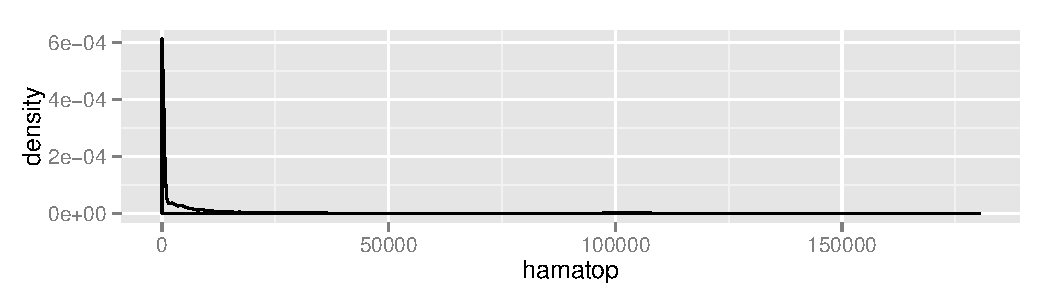
\includegraphics[width=\maxwidth]{figure/addfigure6-1} 

}

\caption[Density plot of hamatop]{Density plot of hamatop}\label{fig:addfigure6}
\end{figure}


\end{knitrout}

\begin{knitrout}
\definecolor{shadecolor}{rgb}{0.969, 0.969, 0.969}\color{fgcolor}\begin{figure}[h!]

{\centering 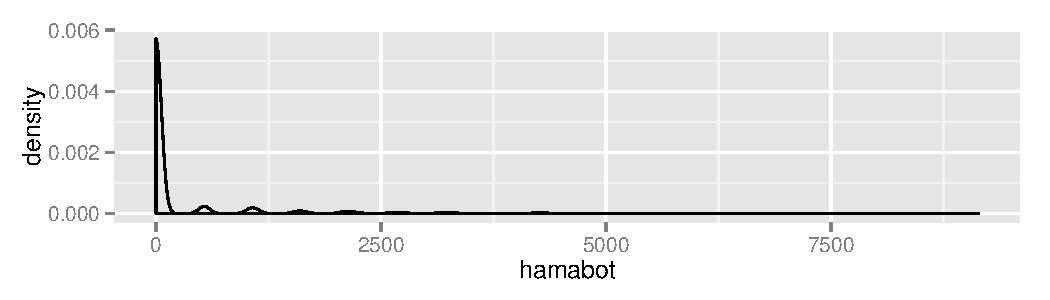
\includegraphics[width=\maxwidth]{figure/addfigure7-1} 

}

\caption[Density plot of hamabot]{Density plot of hamabot}\label{fig:addfigure7}
\end{figure}


\end{knitrout}

\begin{knitrout}
\definecolor{shadecolor}{rgb}{0.969, 0.969, 0.969}\color{fgcolor}\begin{figure}[h!]

{\centering \includegraphics[width=\maxwidth]{figure/addfigure8-1} 

}

\caption[Density plot of hamabot]{Density plot of hamabot}\label{fig:addfigure8}
\end{figure}


\end{knitrout}

Second, after understanding the range of each variables, we want to explore those variables over epoch which we can understand how those variables change over time. We actually cannot really clear see any relationship clearly just by these graphs. Only thing we can know is that those patterns cycled similar through each day.
Probably we need to add height into account.
\begin{knitrout}
\definecolor{shadecolor}{rgb}{0.969, 0.969, 0.969}\color{fgcolor}\begin{figure}[h!]

{\centering \includegraphics[width=\maxwidth]{figure/addfigure9-1} 

}

\caption[Scatter plot of temperature over time]{Scatter plot of temperature over time}\label{fig:addfigure9}
\end{figure}


\end{knitrout}

\begin{knitrout}
\definecolor{shadecolor}{rgb}{0.969, 0.969, 0.969}\color{fgcolor}\begin{figure}[h!]

{\centering \includegraphics[width=\maxwidth]{figure/addfigure10-1} 

}

\caption[Scatter plot of humudity over time]{Scatter plot of humudity over time}\label{fig:addfigure10}
\end{figure}


\end{knitrout}

\begin{knitrout}
\definecolor{shadecolor}{rgb}{0.969, 0.969, 0.969}\color{fgcolor}\begin{figure}[h!]

{\centering \includegraphics[width=\maxwidth]{figure/addfigure11-1} 

}

\caption[Scatter plot of hamatop over time]{Scatter plot of hamatop over time}\label{fig:addfigure11}
\end{figure}


\end{knitrout}

\begin{knitrout}
\definecolor{shadecolor}{rgb}{0.969, 0.969, 0.969}\color{fgcolor}\begin{figure}[h!]

{\centering \includegraphics[width=\maxwidth]{figure/addfigure12-1} 

}

\caption[Scatter plot of temperature over time]{Scatter plot of temperature over time}\label{fig:addfigure12}
\end{figure}


\end{knitrout}

Third, we took height of nodes into account and plotted a series of spatial trends from figure 13 to figure 16. As we can see that once the height of node is high, the variablity is also high as well. it probably because the climate varied a lot in higher height. This situation actually raised my curiosity that if with higher variance in higer location, the equitment would be quickly out of service. I will research on it a little bit in finding section.


\begin{knitrout}
\definecolor{shadecolor}{rgb}{0.969, 0.969, 0.969}\color{fgcolor}\begin{figure}[h!]

{\centering \includegraphics[width=\maxwidth]{figure/addfigure13-1} 

}

\caption[Scatter plot of temperature over height]{Scatter plot of temperature over height}\label{fig:addfigure13}
\end{figure}


\end{knitrout}

\begin{knitrout}
\definecolor{shadecolor}{rgb}{0.969, 0.969, 0.969}\color{fgcolor}\begin{figure}[h!]

{\centering \includegraphics[width=\maxwidth]{figure/addfigure14-1} 

}

\caption[Scatter plot of humidity over height]{Scatter plot of humidity over height}\label{fig:addfigure14}
\end{figure}


\end{knitrout}

\begin{knitrout}
\definecolor{shadecolor}{rgb}{0.969, 0.969, 0.969}\color{fgcolor}\begin{figure}[h!]

{\centering 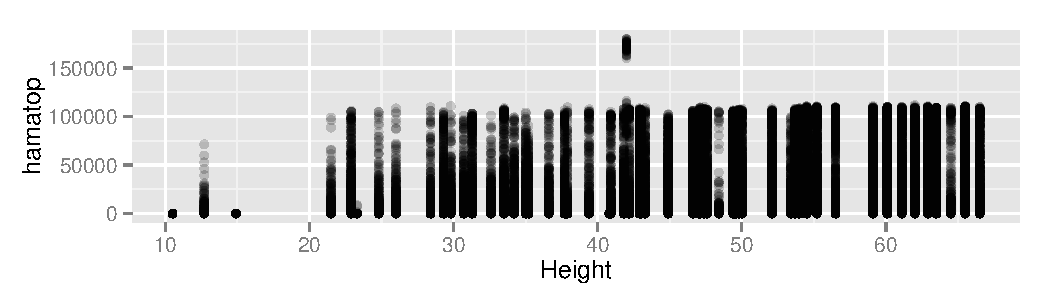
\includegraphics[width=\maxwidth]{figure/addfigure15-1} 

}

\caption[Scatter plot of hamatop over height]{Scatter plot of hamatop over height}\label{fig:addfigure15}
\end{figure}


\end{knitrout}


\begin{knitrout}
\definecolor{shadecolor}{rgb}{0.969, 0.969, 0.969}\color{fgcolor}\begin{figure}[h!]

{\centering 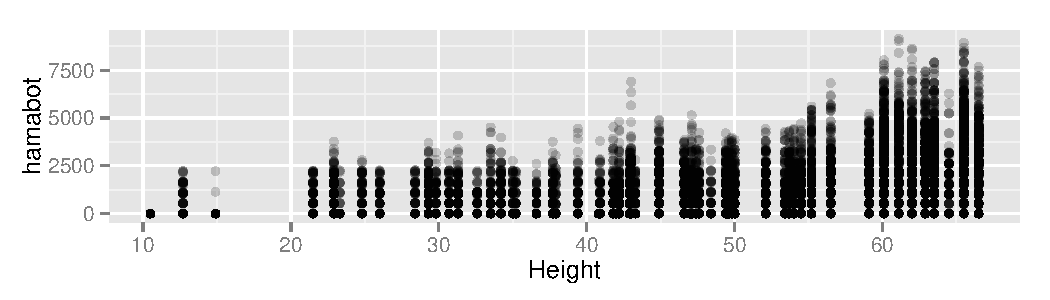
\includegraphics[width=\maxwidth]{figure/addfigure16-1} 

}

\caption[Scatter plot of hamabot over time]{Scatter plot of hamabot over time}\label{fig:addfigure16}
\end{figure}


\end{knitrout}

Lastly, we used colour to diffrentiate the data under different height. For temperature, we can observe that
higer temperature clustered around higher height while it showed oppositely for humidity, higher humidity clustered around lower height. For both PAR, we can also clearly see that higher PAR clustered around the higer location.
\begin{knitrout}
\definecolor{shadecolor}{rgb}{0.969, 0.969, 0.969}\color{fgcolor}\begin{figure}[h!]

{\centering \includegraphics[width=\maxwidth]{figure/addfigure17-1} 

}

\caption[Scatter plot of temperature over time with height]{Scatter plot of temperature over time with height}\label{fig:addfigure17}
\end{figure}


\end{knitrout}

\begin{knitrout}
\definecolor{shadecolor}{rgb}{0.969, 0.969, 0.969}\color{fgcolor}\begin{figure}[h!]

{\centering \includegraphics[width=\maxwidth]{figure/addfigure18-1} 

}

\caption[Scatter plot of humidity over time with height]{Scatter plot of humidity over time with height}\label{fig:addfigure18}
\end{figure}


\end{knitrout}

\begin{knitrout}
\definecolor{shadecolor}{rgb}{0.969, 0.969, 0.969}\color{fgcolor}\begin{figure}[h!]

{\centering \includegraphics[width=\maxwidth]{figure/addfigure19-1} 

}

\caption[Scatter plot of hamatop over time with height]{Scatter plot of hamatop over time with height}\label{fig:addfigure19}
\end{figure}


\end{knitrout}

\begin{knitrout}
\definecolor{shadecolor}{rgb}{0.969, 0.969, 0.969}\color{fgcolor}\begin{figure}[h!]

{\centering \includegraphics[width=\maxwidth]{figure/addfigure20-1} 

}

\caption[Scatter plot of hamabot over time with height]{Scatter plot of hamabot over time with height}\label{fig:addfigure20}
\end{figure}


\end{knitrout}
\section{Graphical Critque}
I thought it's good and starghtforward to present the distributions of each variable at first time. Since distribution plots really gave us the first view of how our data behaved. Take an example, Incident PAR plot in 3(a) distributed as bimodal which probably can explain by full sun and no sun situation are longer than the transition between those. Hence, even though there are probabaly some confounders behind the scene if we only look one dimension plot to make asuumption, 3(a) still provide a good way for us to investigate the dataset. However, on the other hand, I think choosing bins could be an issue for histogram. It could change a lot once the definition of bin change. Like the density plots I showed above, it actually showed different shape of distribution of temperature and humidity. Hence I think it's better to specify the definition of bins.\\

For figure 3(a) and 3(b) I felt it's not really well-illustrative using box-plot in a small graph. it's crowded and very hard to read the trend especially in both PAR graphs. I will probabaly replace it with bigger figure instead of 4 graphs in a line at same time. \\

For figure 4, I thougt it's very clear to illustrate the relationship of temporal trend and spatial trend using this way. it actually limited the effect of confoundder for each snapshot. However, it's not imformative if we want to inspect the whole time instead just a snapshot of one timestep. But the authors fixed it using figure 5.\\

Based on these figures, the authors explained some phenomenons like the temperature in lower trunk is lower than the one in higher trunch while the humidity goes in opposite way or like the node on higher location usually have larger impact regarding to climate changes. However, it also raised some questions at the same time when they addressed some issues. In the context, the authors tries to examine the big dip using figure 4 and 5, they addressed the issue that the node on higher location usually have larger impact regarding to climate changes but we still cannot explain what made the big dip suddenly.

\section{Finding}
At the section of data cleaning, we cleaned a lot of NA readings from the whole dataset. After investigating, I found that those NA comes from the readings of nodeid 15, 122 and 128 which were all located in higer location of the tree. Furthemore, we also observed that data usually have higher variance of microclimate in higher locations in data exploration section. Hence, I was wonder if high variance of data caused those mote to act awry. So I split data into those generated by higer location(larger than 45m) and those generated by lower location(lower than 45m) and checked their box plot of each interested variables. Based on the plots below, we can find that even though temperature's variance in higher location was suprisingly lower than lower locations, there were some points that temperature were higer than 30 degree which could cause the damage of those node. And for both PAR plots, it shows that higher variance in higher locations as we expected. Hence, my finding was that higher temperature and higher variance of intensity of sunlight could probably cause the mote to act awry.
\begin{knitrout}
\definecolor{shadecolor}{rgb}{0.969, 0.969, 0.969}\color{fgcolor}\begin{figure}[h!]

{\centering 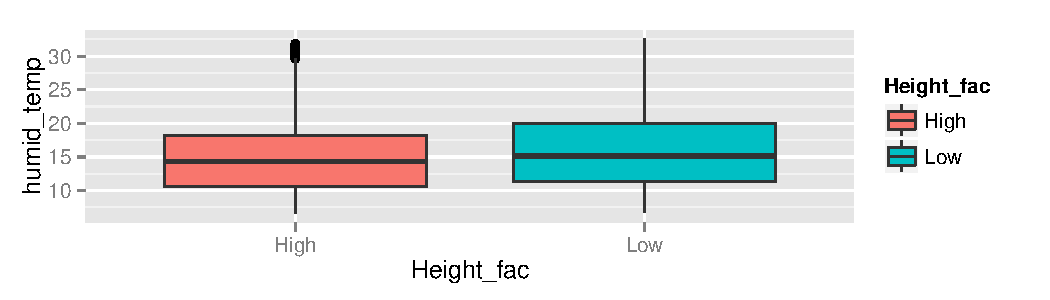
\includegraphics[width=\maxwidth]{figure/addfigure21-1} 

}

\caption[Box plot of temperature over higer locations and lower locations]{Box plot of temperature over higer locations and lower locations}\label{fig:addfigure21}
\end{figure}


\end{knitrout}

\begin{knitrout}
\definecolor{shadecolor}{rgb}{0.969, 0.969, 0.969}\color{fgcolor}\begin{figure}[h!]

{\centering 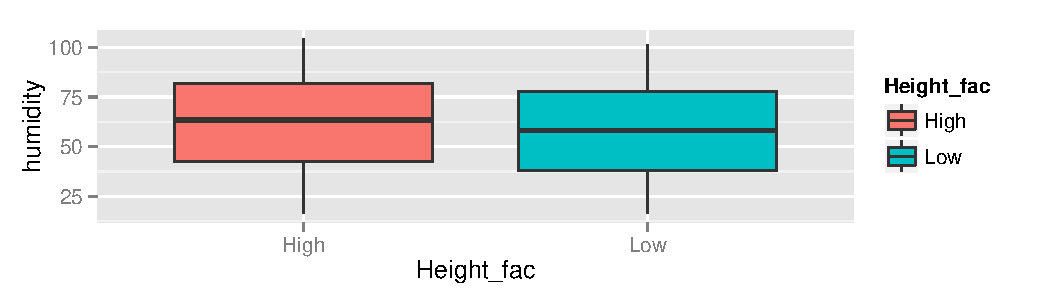
\includegraphics[width=\maxwidth]{figure/addfigure22-1} 

}

\caption[Box plot of humidity over higer locations and lower locations]{Box plot of humidity over higer locations and lower locations}\label{fig:addfigure22}
\end{figure}


\end{knitrout}

\begin{knitrout}
\definecolor{shadecolor}{rgb}{0.969, 0.969, 0.969}\color{fgcolor}\begin{figure}[h!]

{\centering 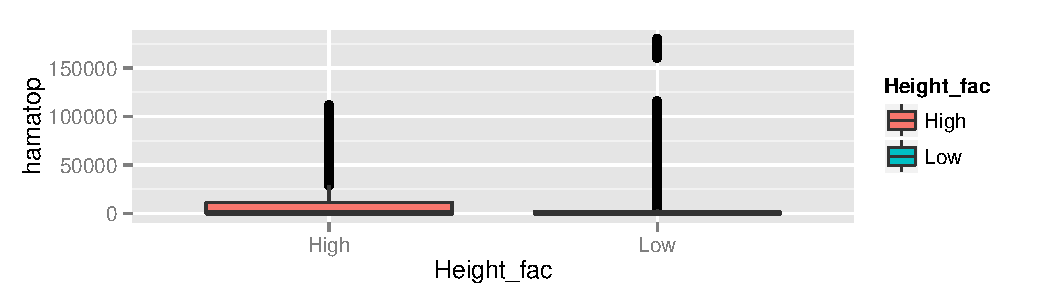
\includegraphics[width=\maxwidth]{figure/addfigure23-1} 

}

\caption[Box plot of hamatop over higer locations and lower locations]{Box plot of hamatop over higer locations and lower locations}\label{fig:addfigure23}
\end{figure}


\end{knitrout}

\begin{knitrout}
\definecolor{shadecolor}{rgb}{0.969, 0.969, 0.969}\color{fgcolor}\begin{figure}[h!]

{\centering 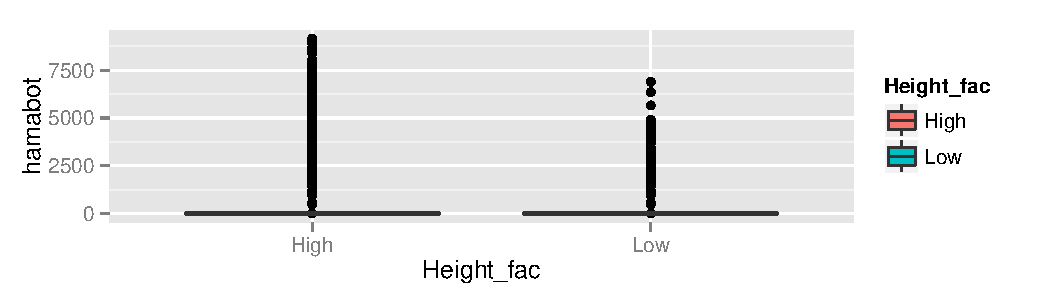
\includegraphics[width=\maxwidth]{figure/addfigure24-1} 

}

\caption[Box plot of hamabot over higer locations and lower locations]{Box plot of hamabot over higer locations and lower locations}\label{fig:addfigure24}
\end{figure}


\end{knitrout}

\section{discussion}
It's pretty challenging to analyze such a raw data with duplicates and missing values at the same time. Aside from this, it also needs to spend a lot of time understanding other people's domain knowledge. Also, for the apsect of the visulization, the trends are always diluted while we represent the graph in 2-D. 2-D plots somehow limited the intepretation of the phenomenon which I think we can use 3-D plots or more interactive graph to address this problem in the future.

\section{conclusion}
Actually, I felt pretty sad that my finding could be dug more deeply and persuasive. I also felt that I spent a lot of time trying to figure out where I should get started to deal with the data. Before this course, I got used to being guided by the instructions which tell us what to do and then we can find those designed answers. However, in this lab, I usually have no lead about what to do. But it was still fun.

\end{document}
